\section{Overview}\label{subsec:overview}

This section starts by motivating the problem of boilerplate code in
traversals of complex structures. It then shows how \name addresses
the problem using a combination of object algebras~\cite{bruno12oa}
and Java annotations.


%Thus we introduce generic queries and transformations to make traversal code reusable and modular. Finally we present our framework \name which a%utomatically generate generic queries, generalized generic queries, transformations and contextual aware transformations based on Object Algebra Int%erfaces with Java annotation.

\subsection{A Company Structure and an Object Oriented Solution}

\begin{figure}[t]
\centering
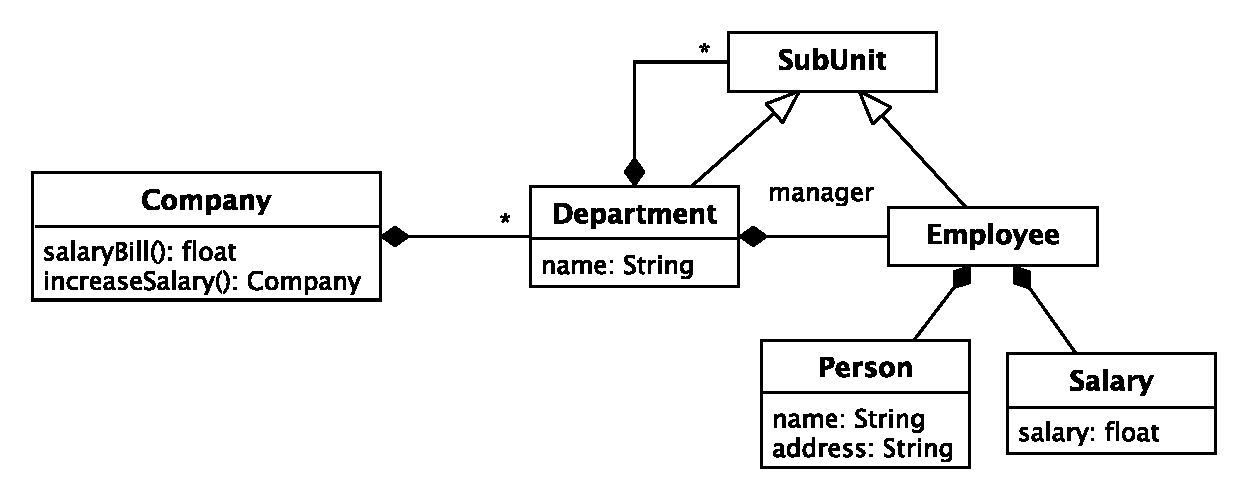
\includegraphics[width=0.9\linewidth]{101companies}
\caption{Variant of the 101 Companies data model\label{company_structure}}
\end{figure}

We start by considering the company structure introduced in
Figure~\ref{company_structure}. The example is inspired by L\"ammel
and Peyton Jones company structure, used to motivate their ``Scrap
your Boilerplate'' approach~\cite{ralf03syb}. It is also closely
related to the 101 companies system~\cite{Inauguration101}.  A
\lstinline{Company} comprises a list of \lstinline{Department}s. Each
\lstinline{Department} is managed by an \lstinline{Employee}, and
contains a list of \lstinline{SubUnits}. A \lstinline{SubUnit} can be
either a \lstinline{Department} or an \lstinline{Employee}. An
\lstinline{Employee} is a \lstinline{Person} with an associated
\lstinline{Salary} information.

\begin{figure}[tb]
\lstinputlisting[linerange=7-24]{../ObjectAlgebras/src/sybDemo1/Company.java} % APPLY:linerange=OOP_COMPANY
\vspace{-.1in}
\caption{The \lstinline{Company} and \lstinline{Salary} classes
  implementing part of the company structure.}
\label{oop_company}
\end{figure}

Two operations are supported by the company structure: querying the
salary bill for the whole company; and increasing the salary of each
employee by 10\%. To support those operations, an OO solution is to
have methods \lstinline{salaryBill}, which returns salary as a float
number, and \lstinline{increaseSalary}, which constructs a company
with updated salaries.

Figure~\ref{oop_company} shows the Java implementation of the
\lstinline{Salary} and \lstinline{Company} classes. The implementation
of other classes is ommitted for space reasons.  In the
implementation, querying the salary bill of the whole company is done
by returning the salary in instances of the \lstinline{Salary} class,
and delegating the method \lstinline{salaryBill} to the child nodes in
other classes. Increasing the salary for the whole company by 10\%,
following L\"ammel and Peyton Jones approach, can be implemented
similarly. The \lstinline{Salary} class will construct a new
\lstinline{Salary} object with increased salary information, and
the method \lstinline{increaseSalary} in classes will
construct corresponding new objects with updated salaries.

\begin{comment}
Just as in functional programming, modelling such company structure in
a conventional OO way leads to significant amounts of boilerplate
code. Object algebras provide an alternative way to model the company
structure, with benefits in terms of extensibility, but there is still
boilerplate code.
\end{comment}

However, this simple OO solution has two important problems:

\begin{enumerate}

\item {\bf Lack of extensibility} The OO style
  representation of data structures is cumbersome and
  inflexible due to the bound relationship between classes. For
  instance, adding a new operation such as pretty
  printing the company structure requires pervasive changes across all
  existing classes.

\item {\bf Boilerplate traversal code} Another issue is that we
  usually need to write a large amount of boilerplate code to
  implement traversals. In our example, we implemented
  \lstinline{increaseSalary} and \lstinline{salaryBill} in all
  classes. However only the \lstinline{Salary} class does some
  interesting work. All other classes simply delegate the task to the
  child nodes. This problem becomes more severe with bigger tree
  structures. The interesting code can become a very small portion of
  the code needed to perform a traversal: most of the code is doing
  tedious walking of the structure.

\end{enumerate}

\subsection{Modeling the Company Structure with Object Algebras}

Object algebras~\cite{bruno12oa} provide a solution to the extensibility problem.
Object algebras are a design pattern that is useful to model complex
structures, while providing a lot of flexibility in terms of
modularity and extensibility. In particular, object algebras allow
extensibility in two dimensions: it is easy to add new types of
nodes; and new operations over the structure.
%As a result, object
%algebras provide a solution to the \emph{expression problem}~\cite{wadler98expression-problem}.

\begin{figure}[tb]
\lstinputlisting[linerange=8-17]{../ObjectAlgebras/src/trees/SybAlg.java} % APPLY:linerange=SYB_TREE
\vspace{-.1in}
\caption{Company structure represented by an object algebra interface}
\label{syb_tree}
\end{figure}

Figure~\ref{syb_tree} shows the approach to model the company
structure as an object algebra interface. Each kind of node (for
example \lstinline{Salary} or \lstinline{Company}) is represented as a
type parameter. Each method in the object algebra interface models a
constructor of some node in the company structure. For example the
method \lstinline{C} constructs an instance of a company; whereas the
method \lstinline{S} creates an instance of a salary. From an
object-oriented perspective the methods in the interface are factory
methods. For the reader familiar with functional programming, the
resamblance to constructors of  (a system of) algebraic datatypes should be clear.

Operations are defined by implementing the object algebra interface.
The following code show a partial implementation of the salary bill
operation.

\begin{lstlisting}[numbers=none,mathescape=true]
class SalaryBill implements SybAlg<Float,Float,Float,Float,Float,Float> {
  public Float C(List<Float> depts) {
    return depts.stream().reduce(0.0f, (x, y) -> x + y);
  }
  $...$
  public Float S(float salary) { return salary; }
}
\end{lstlisting}

The \lstinline{SalaryBill} class provides an implementation for each
of the methods in the object algebra interface, which defines the
overall salary bill operation. Since the result of computing the
salary bill is a \lstinline{Float}, all the type parameters are set to
that type. Most of the method implementations simply traverse the
child nodes and accumulate the salaries. That is the case, for
example, for \lstinline{C}. The only method implementation that does
something different is \lstinline{S}, which returns the salary
argument.
%Note that the way operations are deifined with object
%algebras resembles the definition of operations by case analysis in
%functional programming.

For the increase salary operation the result is itself a structure
with all salaries updated. The following code shows part of the
implementation:

\begin{lstlisting}[numbers=none]
class IncreaseSalary<C,D,U,E,P,S> implements SybAlg<C,D,U,E,P,S> {
	public SybAlg<C,D,U,E,P,S> alg;
	public Float C(List<Dept> depts) { return alg.C(depts); }
	...
	public Salary S(float salary) { return alg.S(salary*1.1f); }
}
\end{lstlisting}

The class \lstinline{IncreaseSalary} is parametrized by six types,
which represent the kinds of nodes in the company structure. Each
constructor needs to build an instance of the right type of nodes.
Note that, due to the lack of better type-inference in Java, there is
some repetition of type-annotations. In order to create the updated
company structure another algebra called \lstinline{alg} is used.
Almost all the method implementations reconstruct the structure with
no changes using the methods in \lstinline{alg}. The exception is the
method \lstinline{S} where the structure is also reconstructed, but
the salary is increased by 10\%.

%In the method
%IncreaseSalary will modify an old algebra and return a new algebra
%based on specific implementations. More specifically, the old algebra
%is set as a field in \lstinline{IncreaseSalarySybAlg}, method
%\lstinline{Salary S(float salary)} increases the salary by 10\%, and
%other methods simply delegates to the same methods in the old algebra.

%When programming with Object Algebras, the code can be very generic based on the object algebra interfaces. \lstinline{alg} can be used as an abstract factory to construct algebras, while the algebras can be instantiated by specific object algebras later by passing in type parameters.

Although we solved the problem of extensibility with object
algebras, the traversal code is still lengthy and we are still writing
tedious traversal code. In both operations, the only interesting code
is in the \lstinline{S} method. Ideally, we would like to write only
the code for the interesting cases, and somehow ``inherit'' the
remainder tedious traversal code.

%It will be better if we can
%design some generic classes for queries and transformations. Hence
%specific algebras can be generated by implementing interesting cases
%of generic queries and transformations. Moreover, it will be even
%better if the boilerplate code can be generated automatically so we
%can focus our attention on the interesting cases.

\subsection{\Name: An Object Algebra Framework for Traversals}


\begin{comment}
Motivated by this problem of writing generic code for tree structure
traversals, we introduce generic queries, generalized generic queries,
transformations and contextual aware transformations with Object
Algebras, which can be easily inherited by real cases of queries and
transformations. Furthermore, we designed an object algebra framework
\name. With our framework, the generic query and transformation
classes can be generated automatically by adding an ``$@$Algebra''
annotation.
\end{comment}

To deal with the boilerplate problem we created \Name: a Java object
algebras framework, which provides a number of generic traversals at
the cost of a simple annotation. The key idea in \name is to
automatically create highly generic object algebras, which encapsulate
common types of traversals. In particular \name supports generic
\emph{queries} and \emph{transformations}. Those two types of
traversals are useful to capture, respectively, the salary bill and
increase salary operations.

With \Name, programmers just need to add an ``$@$Algebra'' annotation
to the definition of \lstinline{SybAlg} to get the code for generic
queries and transformations. An example of that annotation is already
shown in Figure~\ref{syb_tree}. With that annotation several classes
are generated automatically, including \lstinline{SybAlgQuery} and
\lstinline{SybAlgTrans}. Using those classes the code needed to write
the salary bill and increase salary object algebras is much
shorter. The code for the two operations is shown in
Figure~\ref{query_with_oaframework}. By implementing the
\lstinline{SybAlgQuery} and \lstinline{SybAlgTrans} classes, only the
\lstinline{S} method needs to be overriden: all the other methods,
which do a simple generic traversal, are inherited. For queries the
only extra thing a programmer has to do is to provide an instance of a
monoid, which is used to specify how to accumulate the results during
the traversal. Similarly, for transformations, the programmer needs to
pass an algebra for providing the constructors for the transformation
code.

\begin{figure}[tb]
\lstinputlisting[linerange=8-11]{../ObjectAlgebras/src/example_SybAlg/SalaryBill.java} % APPLY:linerange=QUERY_WITH_OAFRAMEWORK
\lstinputlisting[linerange=7-10]{../ObjectAlgebras/src/example_SybAlg/IncreaseSalary.java} % APPLY:linerange=TRANSFORM_WITH_OAFRAMEWORK
\vspace{-.1in}
\caption{Salary bill and increase salary with \Name.}
\label{query_with_oaframework}
\end{figure}

\begin{comment}
\begin{figure}[tb]

\vspace{-.1in}
\caption{Increase salary with \Name.}
\label{transform_with_oaframework}
\end{figure}\bruno{Should we create a simple auxiliary class to make
  the code shorter?}\bruno{I think it is better to merge the 2 figures
(for queries and transformations) into a single figure.}
\end{comment}

Some client code is shown as follows: %, using those two algebras based on our framework.

\lstinputlisting[linerange=12-21]{../ObjectAlgebras/src/example_SybAlg/SybTest.java} % APPLY:linerange=GEN_COM

This method is used to create a particular company structure, in the
usual object algebras style. 
Using this company structure, we can use the \lstinline{SalaryBill}
and \lstinline{IncreaseSalary} to compute some information about the company:

\lstinputlisting[linerange=27-30]{../ObjectAlgebras/src/example_SybAlg/SybTest.java} % APPLY:linerange=CLIENTCODE_COMPANY

The results give \lstinline{111000.0} and \lstinline{122100.0}, which
is respectively the salary before and after increase.

The remainder of the paper provides the details and implementation
techniques used in \Name. Besides basic queries and transformations,
\name also supports two generalizations of these types of traversals
called \emph{generalized queries} and \emph{contextual transformations}.
